\documentclass[11pt]{report}
\usepackage{amsmath}
\usepackage{graphicx}
\usepackage{fancyhdr} % Headers and footers
\pagestyle{fancy} % All pages have headers and footers
\fancyhead{} % Blank out the default header
\fancyfoot{} % Blank out the default footer
\fancyhead[C]{Myocardial Necrosis $\bullet$ BIO4134 $\bullet$ Shifman \& Cole} % Custom header text
\fancyfoot[RO,LE]{Page \thepage} % Custom footer text

\graphicspath{ {/Users/Chris/repos/modeling_final/TeX/images/} } % hard coded mine, sorry about that



\title{\vspace{-15mm}\fontsize{24pt}{10pt}\selectfont\textbf{Extending the Fitzhugh Nagumo Excitable Tissue
Model to Myocardial Necrosis}} % Article title

\author{
\large
\textsc{Aaron R. Shifman, Christopher B. Cole}\thanks{BIO4134 Final Project}\\[2mm] % Your name
\normalsize University of Ottawa \\ % Your institution
\vspace{-5mm}
}
\date{}

%----------------------------------------------------------------------------------------

\begin{document}

\maketitle % Insert title

\thispagestyle{fancy} % All pages have headers and footers

%\tableoffigures

\begin{abstract}

Neuroscience frequently relies on robust mathematical models to simulate and investigate trends in neuromechanics and signal propagation. We propose an examination of the Fitzhugh-Nagumo model, and additionally propose a modified extension of this model to account for necrosis of cardiac cells. We use this model to investigate case studies in cardiac necrosis and examine the effect of necrosis on a one dimensional cardiac model. 
\end{abstract}


\newpage

\tableofcontents

\newpage

\chapter{Examination of the Fitzhugh Nagumo Model}

The modelling of neurons and associated action potentials started in the early 1900s with the ``integrate and fire'' model.$^1$ In 1952, Hodgkin and Huxley created a biologically relevant 4 dimensional system of equations to describe neuron dynamics at a point.$^2$ While very interesting to biologists, mathematicians found the model too difficult to systematically study. In 1961 Richard Fitzhugh created a 2D caricature of the Hodgkin Huxley model (activation and recovery) using a modified Van-der-Pol oscillator.$^3$ This model has been both well studied and well characterized. Additionally, it has found many uses in cardiac models due to its simplicity and similarity in shape to a cardiac action potential. 

The Hodgkin Huxley equations described how neuronal membrane voltage changed over time, given a large number of parameters. 

\begin{align}
C_m \frac{dV}{dt} &= I_m = I_{Na} + I_{K} + I_l \\
I_x &= \bar{G_x}p_{open}(V_m-E_x); x\in\{Na,K,l\}\\
p_{open_{K}} &= n^4\\
p_{open_{Na}} &= m^3h\\
p_{open_{l}} &\equiv 1\\
\frac{dx}{dt} &= \alpha_x(V)(1-x)-\beta_x(V)x; x\in{m,n,h}\\
\end{align}

This is impossible to solve analytically, and quite difficult to explore numerically due to the high dimensionality of the system and the large number of parameters. In studying hyperplanes through the 4D phase space, Nagumo noticed that all planes of activation and recovery variables had a similar shape, so he tried modeling neuronal activity as a modified Van-der-Pol oscillator (Bonheffer-Van-der-Pol oscillator). This model, while not looking like stereotyped action potentials, has several features of the full hodgkin huxley model such as activation hysteresis and spike blocking. Despite not looking like a neuronal action potential, it closely resembles cardiac action potentials and have since been adapted as one of the de-facto models for cardiac simulations. 


\section{Model Rationale and Variables}

The system presents in the following, non-dimensionalized form. This is not the original Bonheffer-Van-der-Pol model, however it is topologically equivalent and much easier to analyse.

\begin{align} \frac{dV}{dt} &= V(\alpha+V)(1-V) -W + z \\
\frac{dW}{dt} &= \beta V-cW \end{align}

In this model, $V$ - in general - represents activation, and in an excitable tissue context represents voltage. and $W$ - in general represents recovery, and has no realistic interpretation in a biological context, it would be the sum of all positive \( W.R.T. cell \) currents. There are three parameters in the model, $\alpha$, $\beta$, $c$, and $z$. Of the three parameters, we have significant interest in $z$, as it will determine the bifurcation of the model. Neurologically, $z$ represents the DC offset from experimentally injected current of the neuron under study. In our extension to this model, we will replace $z$ with a gap junctional current from coupled cells (more in section 2). The additional parameters $\alpha$, $\beta$, and $c$ represent `rate - like' constants which determine oscillator traits such as amplitude, frequency, duty cycle, and excitability.


\section{Purpose of Model and Examination}

This model, a simplification of the original Hodgkin Huxley model, intends to model spiking neurons. Tuning the individual parameters can adapt the model to fit various states and conditions which may be investigated by researchers. Various combinations of parameters can also model neuronal behaviors such as bursting and chattering. These models can be put together to form multi-dimensional models of neuron trends. The state of the neuron relies on the $z$ parameter. 
In this project, we plan to evaluate the stability of system at rest and with regards to the bifurcation parameter $z$. We plan to evaluate how the system responds and bifurcates with regards to this parameter, and interpret these stabilities biologically. 

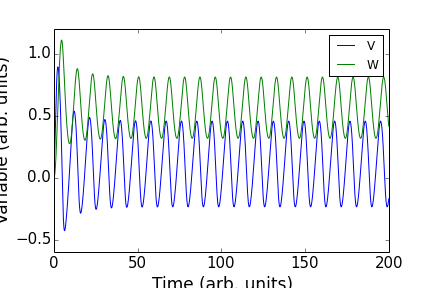
\includegraphics[scale=0.75]{model}


\section{Model Classification} % (fold)
\label{sub:model_classification}

% subsection model_classification (end)

\section{Dimensionalization} % (fold)
\label{sub:dimensionalization}

% subsection dimensionalization (end)
\section{Stability Analysis} % (fold)
\label{sub:stability_analysis}

Taking our model such that:

$$\begin{aligned}
f(x) &= \dot{V} = V(\alpha + V)(1-V) -W +z \\
g(x) &= \dot{W} = \beta V -cW
\end{aligned}
$$

We compute the Jacobian Matrix $\vec{J}$:


$$
\vec{J} = \begin{bmatrix}
    \frac{\partial f}{\partial{V}} & \frac{\partial f}{\partial{W}} \\
    \frac{\partial g}{\partial{V}} & \frac{\partial g}{\partial{W}} \\
\end{bmatrix} = 
\begin{bmatrix}
    −2\alpha V+\alpha+(2 - 3V)V & -1 \\
    \beta & -c \\
\end{bmatrix}
$$


If we take $\alpha,\beta,c$ equal to 0.01,0.5,0.1, we get $\Rightarrow $
$$
\begin{bmatrix}
    −0.02V+(2−3V)V+0.01 & -1 \\
    0.5 & -0.1 \\    
\end{bmatrix}
$$

This implies that eigenvalues $\lambda_{1,2}$ may be complex or not. 

Eigenvalues 1 and 2 as follows

$$ \lambda_{1,2} \approx 0.5(-3V^2 - 1.98V \pm \sqrt{ 9V^4 + 11.88 V^3 + 3.2604 V^2 - 0.4356 V - 1.9879 } - 0.09) $$

with corresponding eigenvectors

$$ v_{1,2} \approx \begin{bmatrix} 0.11 + 1.98V - 3V^2 + \sqrt{ 9V^4 + 11.88 V^3 + 3.2604 V^2 - 0.4356 V - 1.9879} & 1 \\ 0.11 + 1.98V - 3V^2 - \sqrt{ 9V^4 + 11.88 V^3 + 3.2604 V^2 - 0.4356 V - 1.9879} & 1 \end{bmatrix} $$

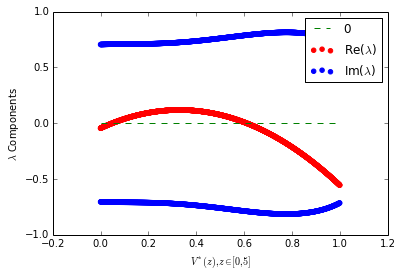
\includegraphics{eig}
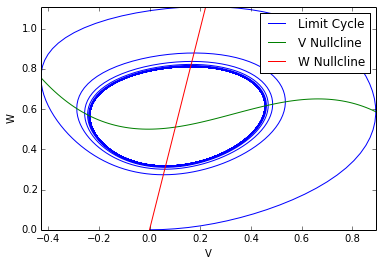
\includegraphics{phase-plane}
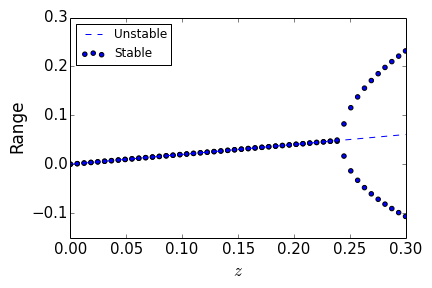
\includegraphics{lbifur}
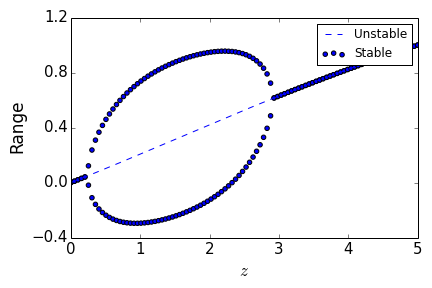
\includegraphics{hbifur}
% subsection stability_analysis (end)




\section{Coupled Oscillators} % (fold)
\label{sub:coupled_oscillators}

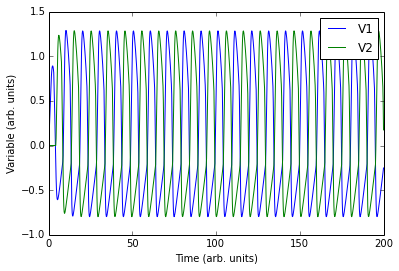
\includegraphics{2couple}
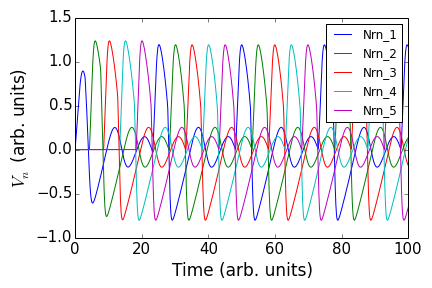
\includegraphics{ncouple}



% subsection coupled_oscillators (end)

%end original model, begin extension

\chapter{Modelling Myocardial Necrosis} 


\section{Translational Perspective} %how the model relates to disease

The heart serves a vital role in many organisms. The timely and regular delivery of oxygenated blood is essential to survival, and thus any decrease from optimum efficiency is of consequence. Investigations into potential mechanistic explainations and modeling of this degradation are highly interesting in the context of both accute and chronic cardiac disease.

In particular, myocardial necrosis can be caused by accute oxygen deprivation of myocardial tissues, commonly experienced during a heart attack. Other potential etiologies stem from depriving this tissue of the blood it requires; dangerous increase in physical stresses, coronary artery disease, and accute hemerage all have the potential to play into cardiac necrosis, perhaps in tandem. 

In our investigation into the decreasing efficiency of a heart-like system, we will model several scenarios that may be of consequence to sufferers of cardiac necrosis. In particular, we study two cases. The first, static necrosis, closely resembles a short term or acute stress on myocardial tissue, be it a myocardial infarction or trauma. We will investigate how the distribution of necrosis affects the system as a whole through the FN model. Through a translation lens, this equates to the decrease in efficiency as a consequence of various kinds of trauma. The second case will be a slowly increasing level of necrosis. This more closely resembles coronary artery disease, which has the potential to starve the tissues of oxygen for many years, slowly leading to health deficits in older age. We study the approximate timeframe for simulated tachycardia, or dangerously low heart beat. 

Throughout the investigation, we refer to a cell's necrosis burden as analagous to a protein build up, though this simply refers to the degree of degredation for that specific cell.

Our proposed extension to the FN model plans to shed light on the geneisis, progression, and finally the consequences of myocardial necrosis. 

\section{Necrosis Propagation}

As part of the normal cell cycle, programmed cell death (apoptosis) exists and it serves several purposes. In most cases, it is both irreversible and adaptive (beneficial) for the organism. However in some cases, apoptosis can occur accidentally in which case an irreversible destruction of the cell will occur. In our model, we assume that necrosis is a function of an underlying accumulation of pro-apoptotic proteins, potentially introduced as a byproduct of disease. As such, necrosis is a continuous state of each cell. For cell $i$ of $n$, define pro-necrotic burden as $\nu_i$, with total burden of the system equal to $\frac{\sum^n_{i=1} \nu_i}{n}=\frac{1}{n} \sum^n_{i=1} \nu_i$. Note that $\nu_{1}, ..., \nu_{n} \in [0,1]$ and is a monotonically increasing function with respect to time. 

Starting with the Fitzhugh Nagumo model equivalent
\begin{align}
\frac{dV}{dt} &= V(\alpha +V)(1-V) -W +z\\
\frac{dW}{dt} &= \beta V - cW
\end{align}
We connect connect oscillators with a gap junctional current ($I_g = G_g(\Delta V)$). For a population of $n$ oscillators $\Omega$, with members $\omega_i; i\in \textbf{N}; 1\leq i\leq n$. If $\omega_i$ is connected to $x; x\subset\Omega$, then the gap junctional current to $\omega_i$ is $\sum_{x} G_{x,i}(V_i-V_x)$

In the case of 2 oscillators ($A$ and $B$)

\begin{align}
\frac{dV_A}{dt} &= V(\alpha +V_A)(1-V_A) -W_A + G_g(V_A-V_B) + z_A\\
\frac{dV_B}{dt} &= V(\alpha +V_B)(1-V_B) -W_B + G_g(V_B-V_A) +z_B\\
\frac{dW_A}{dt} &= \beta V_A - cW_A\\
\frac{dW_B}{dt} &= \beta V_B - cW_B
\end{align}

\section{Diseased States}
For the coupled oscillators representing cardiac myocytes (eq. 3-6), as the cells die through an apoptotic pathway, a fraction of their gap junctions $\nu \in [0,1]$ will be destroyed, through cell decay.

In order to model disease, each myocyte will have a corresponding $\nu$ term, such that

\begin{align}
\frac{dV_A}{dt} &= V(\alpha +V_A)(1-V_A) -W_A + (1-\nu_A) G_g(V_A-V_B) + z_A\\
\frac{dV_B}{dt} &= V(\alpha +V_B)(1-V_B) -W_B + (1-\nu_B) G_g(V_B-V_A) +z_B
\end{align}
With increasing $\nu$, the cell becomes less responsive to its coupled partners

\section{Static Disease Burden} % (fold)
\label{sub:static_disease_burden}

\begin{enumerate}
	\item Does distance (Distance between $N_i$ and $N_j= j -i$) influence $D$
	\item Is $D$ decreased more by a few heavily burdened cells, or by a large number of moderately burdened cells
	\item At what point does the build up of pro-necrotic proteins become a health issue (health being defined such that $T_t \geq kT_n; k\in[0,1]$)
\end{enumerate}

\section{Dynamic Disease Burden} % (fold)
\label{sub:dynamic_disease_burden}

In order to extend this model to model cardiac necrosis, we use the previously described coupling and add $\nu_i$ as an ordinary differential equation describing the dampening on neuron $i$ ($N_i$). In the present simplication, $\nu_i$ will depend only on time. Define $\nu_{0i}$ as the *a priori* necrotic burden of $N_i$. 

We wish to construct a model of $\nu_{i}$ evolution where, eventually, the disease will destroy the cell. Thus, we wish to have 1 (complete dampening) as a stable steady state. Additionally, we require that any concentration of $\nu_{0i}$ will eventually lead to cell death. We chose the model

$$ \frac{d \nu_i}{dt} = \dot{\nu} = \nu_i (1 - \nu_i) $$

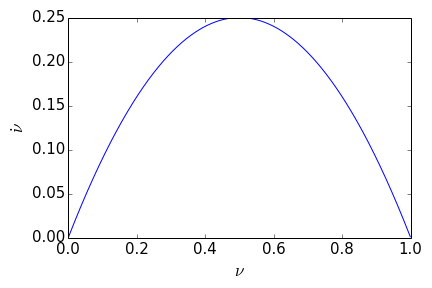
\includegraphics{dynamic}
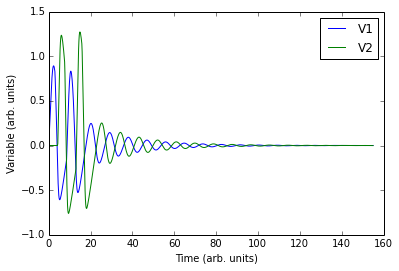
\includegraphics{2dyn}
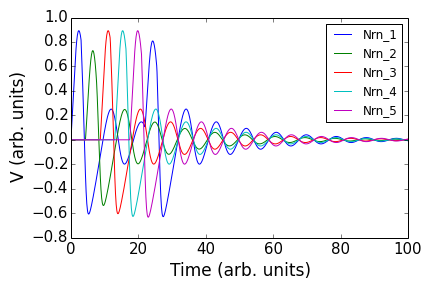
\includegraphics{ndyn}
% subsection dynamic_disease_burden (end)


% subsection static_disease_burden (end)
\section{Web App} % (fold)
\label{sub:web_app}


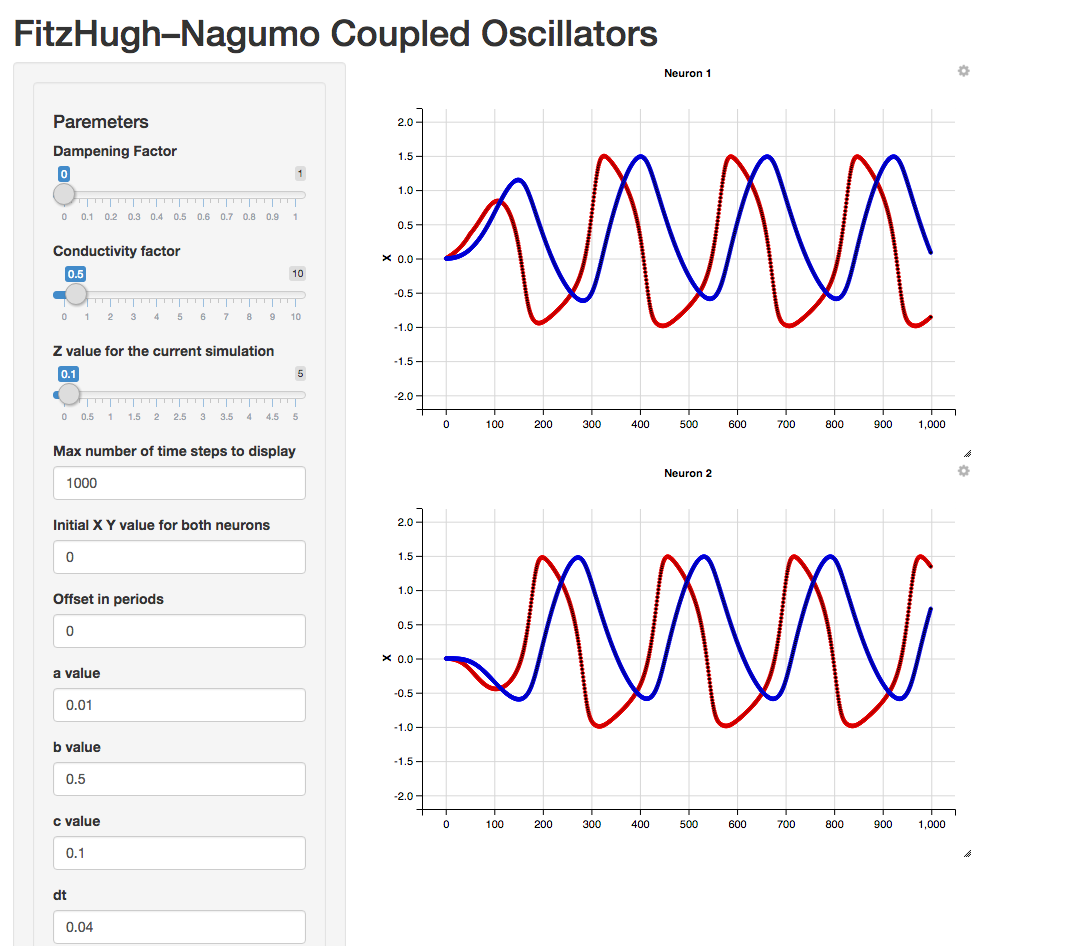
\includegraphics[scale = 0.4]{R}
% subsection web_app (end)
\newpage

\chapter{References} % (fold)
\label{sec:references}

\begin{enumerate}
	\item Abbott, L. . Lapicque’s introduction of the integrate-and-fire model neuron \(1907\). Brain Res. Bull. 50, 303–304 \(1999\).
	\item Hodgkin, A. L., Huxley, A. F. A quantitative description of membrane current and its application to conduction and excitation in nerve. J. Physiol. 117, 500–44 \(1952\).
	\item Haefner, J. W. Models of Systems. Modeling Biological Systems: Principles and Applications \(Springer, 2005\). doi:10.1007/0-387-25012-3\_1
\end{enumerate}


% section references (end)

\end{document}





